%!TEX root = ../dokumentation.tex

\chapter{Ausarbeitung von Lösungen}
\section{Aufbau des Projektes}
Um die Sensordaten bereitzustellen, müssen verschiedene Schritte durchlaufen werden. Zuerst muss eine physikalische Verbindung zum Sensor aufgebaut werden. //TODO

\subsection{Physikalische Verbindung zwischen Sensor und Arduino herstellen (Schaltkreis aufbauen)}
Um die Sensordaten zu ermitteln muss zuerst der Sensor mit dem ESP8266 verbunden werden. Zur Inbetriebnahme des HC-SR04 sind vier Verbindungen notwendig.
\begin{itemize}
    \item VCC: Spannungsversorgung 5V
    \item GND: Masse
    \item Trig: Daten (in)
    \item Echo: Daten (out)
\end{itemize}
Um also die Sensordaten auslesen zu können, wurde der folgende Schaltkreis entwickelt:
\begin{figure}[h!]
	\centering
	\resizebox{.9\textwidth}{!}{%
		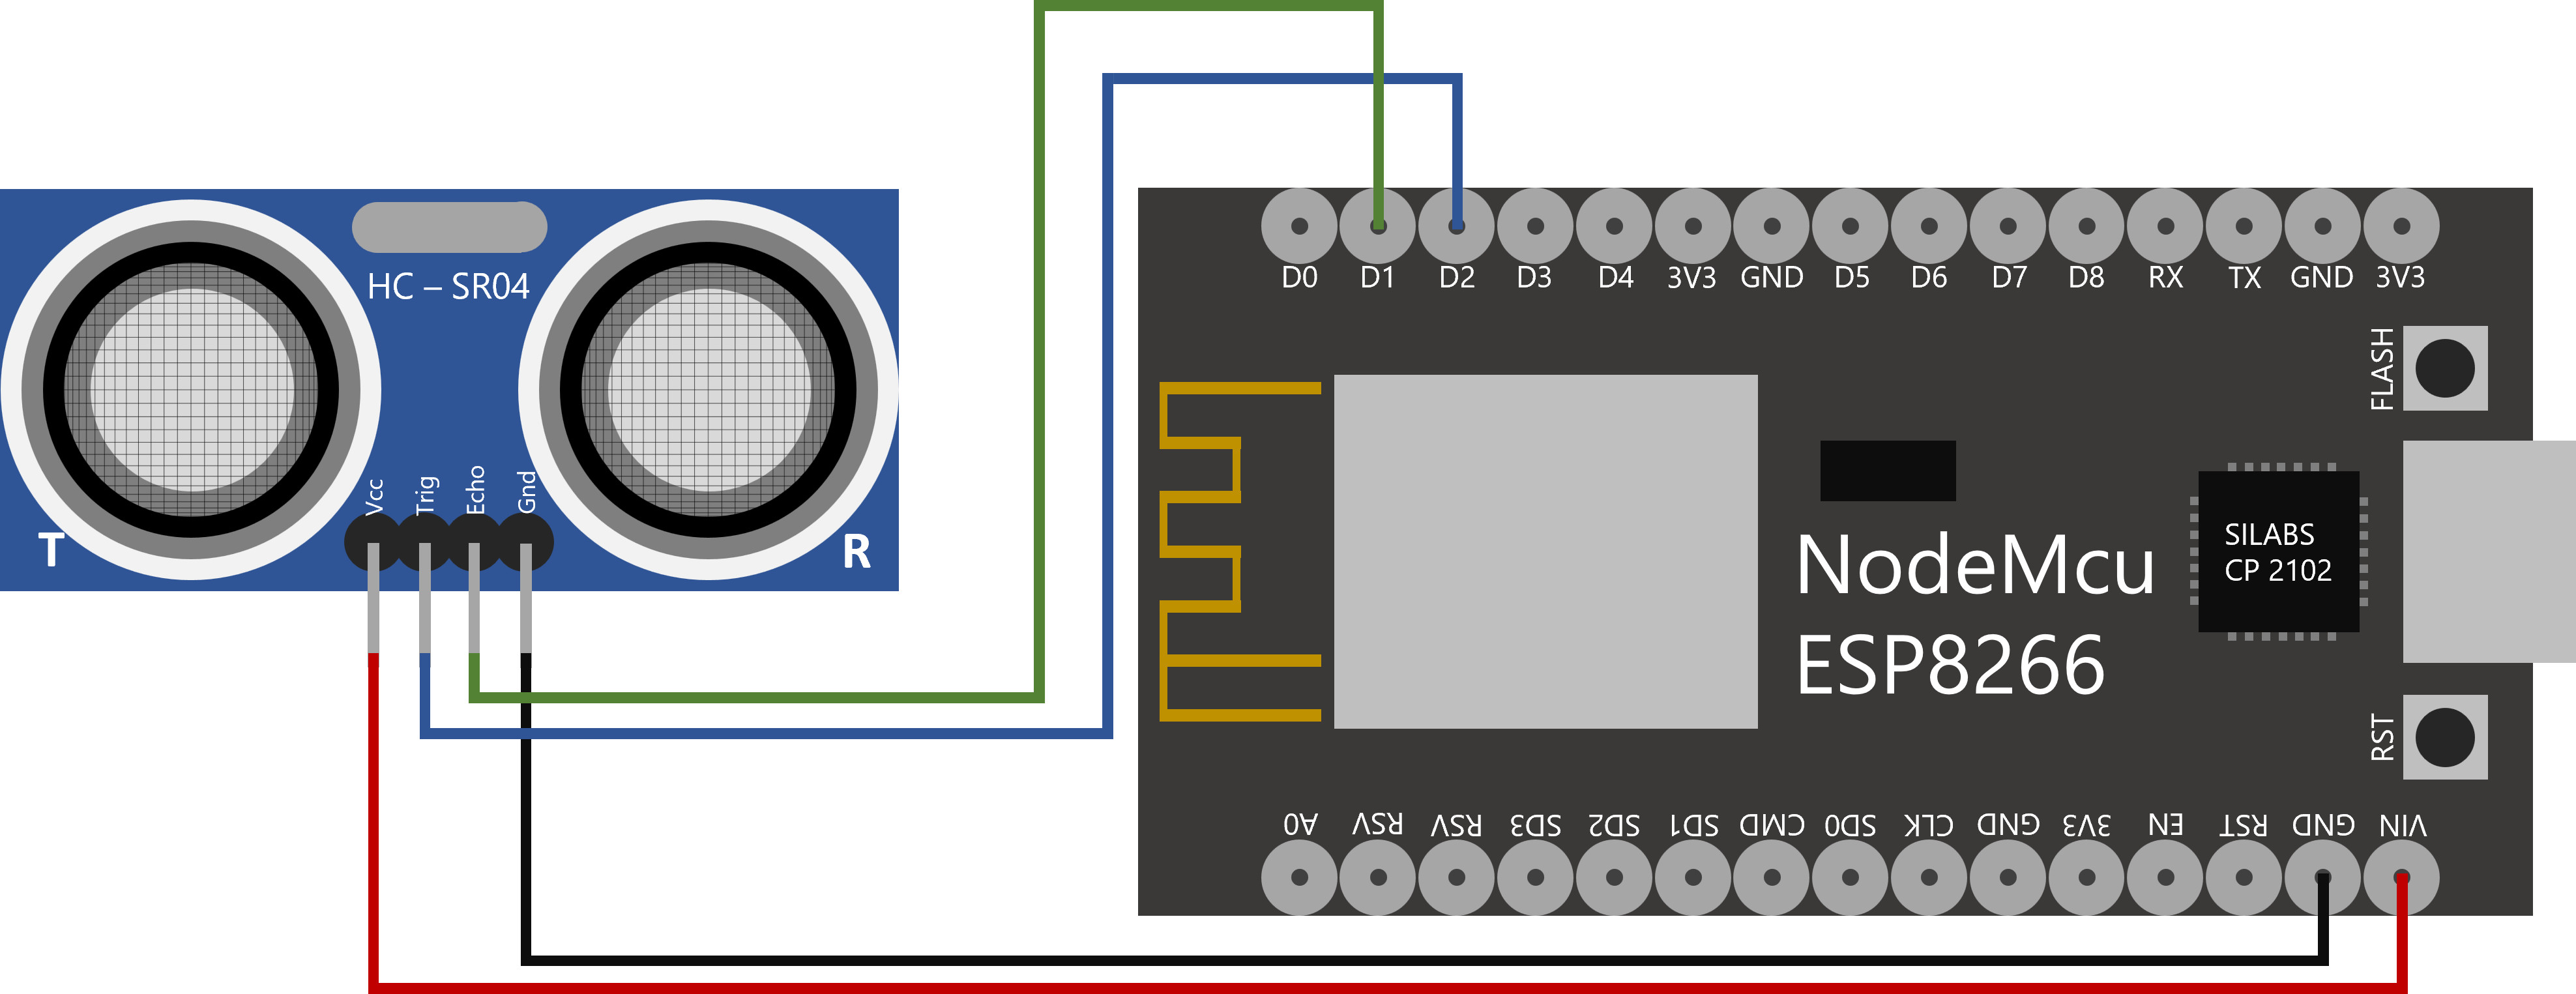
\includegraphics{images/Schaltung.png}
	}
	\caption[Entwickelter Schaltkreis]{Entwickelter Schaltkreis, eigene Darstellung \protect\citeM{i}{IoTspace.dev}{}{}}\label{fig:withSource} % Wie gebe ich hier die Quelle an?
\end{figure}
\subsection{Programmierung zum Ermitteln und Bereitstellen der Sensordaten}
Nachdem die Physikalische Verbindung zum Sensor hergestellt ist und dieser mit Strom versorgt wird, muss noch Programmcode entwickelt werden, welcher die Daten zum richtigen Zeitpunkt anfragt. Damit der ESP möglichst wenig Strom verbraucht und nicht unnötig belastet wird, werden die Daten nur auf Anfrage von Außen ermittelt. Dieses Vorgehen nennt sich auch Datenkapselung. Leider hat es neben den genannten Vorteilen auch einen Nachteil. Die Daten können nämlich nach diesem Prinzip nur aktuell und nicht in die Vergangenheit abgefragt werden. Sollte man sich also für den Verlauf der Daten interessieren, so kann dieser nicht vom ESP geliefert werden. Dieses Problem ist jedoch einfach zu umgehen, indem die Anwendung sich die erhaltenen Sensordaten einfach in einer eigenen Datenbank speichert. Nach dem Start des ESP lässt sich der Vorgang in verschiedene Schritte unterteilen:
\begin{enumerate}
    \item Verbindung mit dem konfigurierten WLAN herstellen
    \item DNS-Eintrag erstellen
    \item NTP-Client erstellen
    \item Server-Endpoints definieren
    \subitem Datenendpunkt (JSON)
    \subitem Websiteendpunkt (HTML)
\end{enumerate}
Nach diesem Aufbau wird beim Start des ESPs nur initialisiert. Nachdem dieser Prozess abgeschlossen ist, kann ein User die Website laden. Diese lässt sich dann über den Data-Entpoint die live-Daten geben und zeigt diese an.
\subsection{Programmierung zum Anzeigen der bereitgestellten Sensordaten}
Um die aktuellen Daten zu visualisieren gibt es verschiedene Möglichkeiten. Beispielsweise bietet \ac{HTML} mit dem 'meta'-Tag eine Möglichkeit zum Aktualisieren der Seite in einem Intervall. Diese Option wäre jedoch sehr unschön, da das Aktualisieren sich statt nur auf die gezeigten Daten auf die gesamte Seite auswirken würde. Eine weitaus schönere Option ist das Aktualisieren der \ac{HTML}-Elemte, in welchem die Daten angezeigt werden. Hierzu muss die angezeigte Seite ein Script enthalten, welches die Daten in einem festgelegten Intervall vom ESP abfragt und dann nur den Inhalt der spezifischen Elemente aktualisiert.
Ich habe mich für die Umsetzung der zweiten Lösung entschieden, da ich so mit einem geringen Mehraufwand eine beträchtliche Verbesserung für den Nutzer erreichen kann. Wenn die Webseite geladen wird, dann wird eine JavaScript Datei mitgegeben. Dieses Skript aktualisiert die angezeigten Werte auf der Website in einem festen Intervall einmalig jede Sekunde.